\subsection{Description of the system}
\begin{figure}[H]
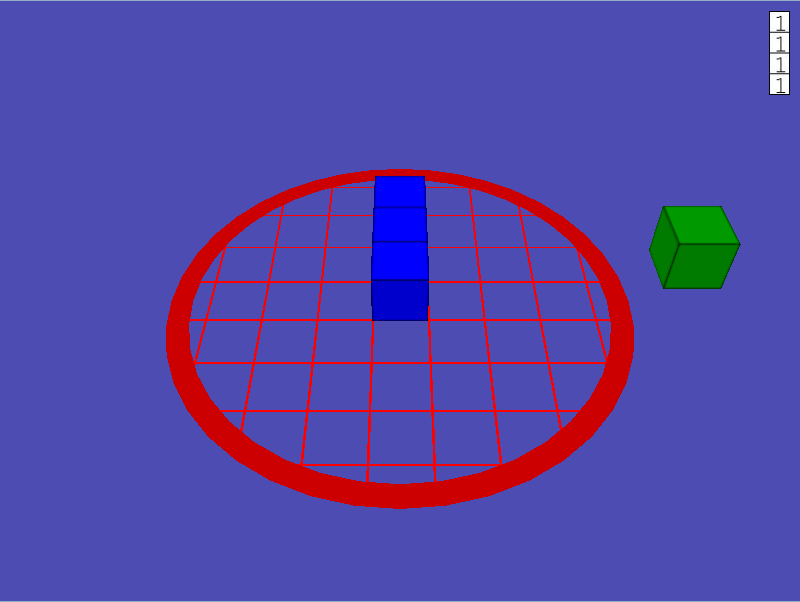
\includegraphics[width=\textwidth]{imgs/environment}
\caption{The environment in which the structures had to be build.}
\label{fig:environment}
\end{figure}

The system build for the experiment consisted of three main parts. First, there was an environment in which the structures could be build (see Figure~\ref{fig:environment}). The environment looked simple. There was a circle with a grid inside in which the structures had to be build. On the right side (or left side for people who were left-handed), there was an infinite stack of blocks. The users of the system could grab here new blocks if they needed them. In the right upper corner there was a representation of the structure that had to be build for the experiment.
% Both the User Interface (UI) and the user interactions were designed to be minimalistic, simple and intuitive in order to prevent users having to learn a lot before they could use the system. 

Next to the environment there were two different interfaces with which you could build in the environment. First, there was a LEAP-motion interface, using hand movements to build the structures. Second, there was a interface which used a combination of the mouse and the keyboard.

In the next section there are more details about how the environment and how the interfaces are implemented.

% Short description of the experimentor interface